% !TeX root = DistributedConsensus.tex
% !TeX spellcheck = en_GB
\chapter{Connecting Histories}\label{chap:connecting-histories}
	In this chapter the representation of histories is used to combine multiple local histories into one global history using the information of actions. Furthermore two approaches to gather histories from the events are described.
    
    \section{Merging Histories}\label{sec:connecting:merge}
    Given the representation of a history, and because the actions of executions are distributed among several events, we need a way to connect the actions by happens-before relations.

	\newpar In order to simplify this problem it is assumed that all local histories are \textit{\textbf{valid}}. That is:
    
    \begin{definition}
    A \textit{\textbf{valid history}} is a history, where all actions happen according to the rules of the DCR graph, abiding serial equivalence and being in strict partial order. Also, a valid history \textbf{must} contain exactly the actions that \textbf{did} happen in the execution of events.
    \label{def:validhistory}
    \end{definition} 

	\noindent The observation and identification of invalid histories are described in \autoref{chap:validation}. Why it is necessary to have this assumption is discussed in the end of this section.

    \newpar Given valid local histories of several events, we want to connect the actions of the histories such that the result has the fewest possible concurrent actions using happens-before relations. Furthermore, given a global history $A$ and every local history $B$ used for the creation of $A$, for every path from action $x$ to another action $y$ in $B$, there must also exist a path from $x$ to $y$ in $A$.
    
    \newpar The concept of happens-before relations, as described in \autoref{subsec:orderingofevents} helps determining which actions have happened before others across events. For each outgoing action in a history, there must be another incoming action, because these actions are the two sides of the same effect. Therefore, each outgoing action type corresponds to an incoming action type by the following definition:
	
	\begin{definition}
		\label{def:happensbeforeaction}
		The action types that \textbf{correspond} are:
			\begin{itemize}
				\item Checks condition $\rightarrow$ Checked condition by
                \item Excludes $\rightarrow$ Excluded by
				\item Includes $\rightarrow$ Included by
				\item Sets pending $\rightarrow$ Set pending by
			\end{itemize}
	\end{definition}
	
	\noindent For any outgoing or incoming action on an event, there might exist any number of actions with corresponding action types. Actions should therefore be matched on more than just their corresponding action type. An action includes the ID and timestamp of both the executing and counterpart event to ensure that matches are unique.
	This brings us to the definition of a \textbf{match}:
    
    \begin{definition}
    	\label{def:action:matching}
    	A pair of actions, $a$ and $b$, \textit{\textbf{match}} if and only if they have corresponding action types and the ID and timestamp of $a$ is identical with the counterpart ID and counterpart timestamp of $b$. Furthermore, the ID and timestamp of $b$ must be identical with the counterpart ID and counterpart timestamp of $a$.
    \end{definition}
    
    \noindent Figure \ref{fig:connect:actions-match} is an example of a pair of matching actions.  In \autoref{fig:connect:actions-do-not-match} the actions do not match.
    
    \begin{figure}[H]
		\centering
		\begin{minipage}{0.45\textwidth}
			\centering
			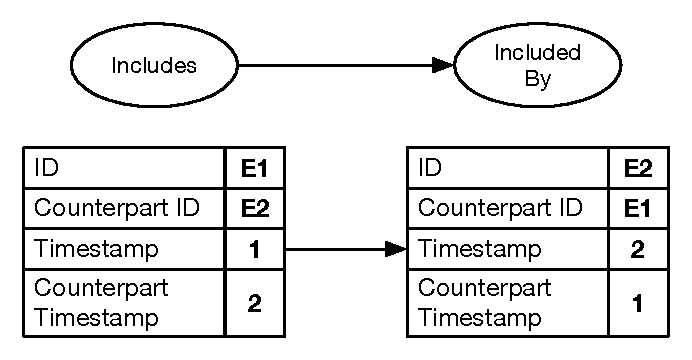
\includegraphics[width=\textwidth]{4connect/images/actions-match.pdf}
			\caption{Two actions that match.}
			\label{fig:connect:actions-match}
		\end{minipage}\hfill
		\begin{minipage}{0.45\textwidth}
			\centering
			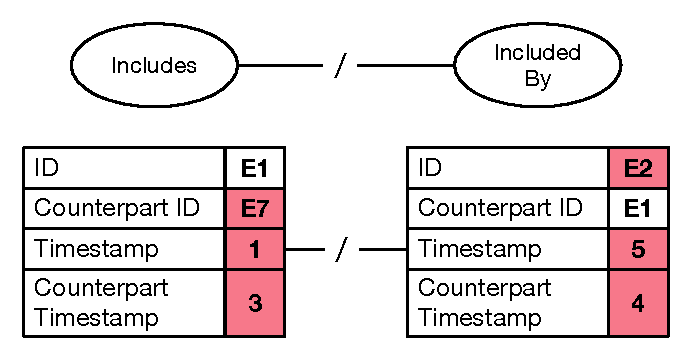
\includegraphics[width=\textwidth]{4connect/images/actions-do-not-match.pdf}
            \caption{Two actions that do not match. Fields that do not match are marked with red.}
            \label{fig:connect:actions-do-not-match}
		\end{minipage}
    \end{figure}
        
    \noindent An outgoing action must happen before its incoming counterpart, because together they represent a message exchange between to processes. A happens-before relation is established between the matching actions represented by adding an edge from the outgoing action to the incoming action in the history.

	\newpar To create a history of the entire set of events, every action of every local history needs to be added to a joined global history. Therefore the algorithm must take a set of local histories and merge them together, two at a time, until one final combined history remains. The \textit{Merge} algorithm is outlined in \autoref{alg:merge}.
	
	\begin{algorithm}[H]
		\begin{algorithmic}
			\Function{Merge}{history1, history2} \textbf{returns} \textit{a merged history}
			\State combinedHistory $\leftarrow$ \Call{UnionNodesAndEdges}{history1, history2}
			\ForAll{action \textbf{in} combinedHistory}
			\If{\Call{IsOutgoing}{action}}
            	\ForAll{action' \textbf{in} combinedHistory}
                	\If{\Call{Matches}{action, action'}}
						\State combinedHistory $\leftarrow$ \Call{AddEdge}{action, action', combinedHistory}                    	
                    \EndIf
                \EndFor
			\EndIf
			\EndFor
			\State\Return combinedHistory
			\EndFunction
		\end{algorithmic}
		\caption{The \textit{\textbf{Merge}} algorithm}
		\label{alg:merge}
	\end{algorithm}
	
    \noindent Figure \ref{fig:connecting:match-before-after} shows the local histories of two events, before and after a matching pair of actions have been found.
    
	\begin{figure}[H]
		\centering
		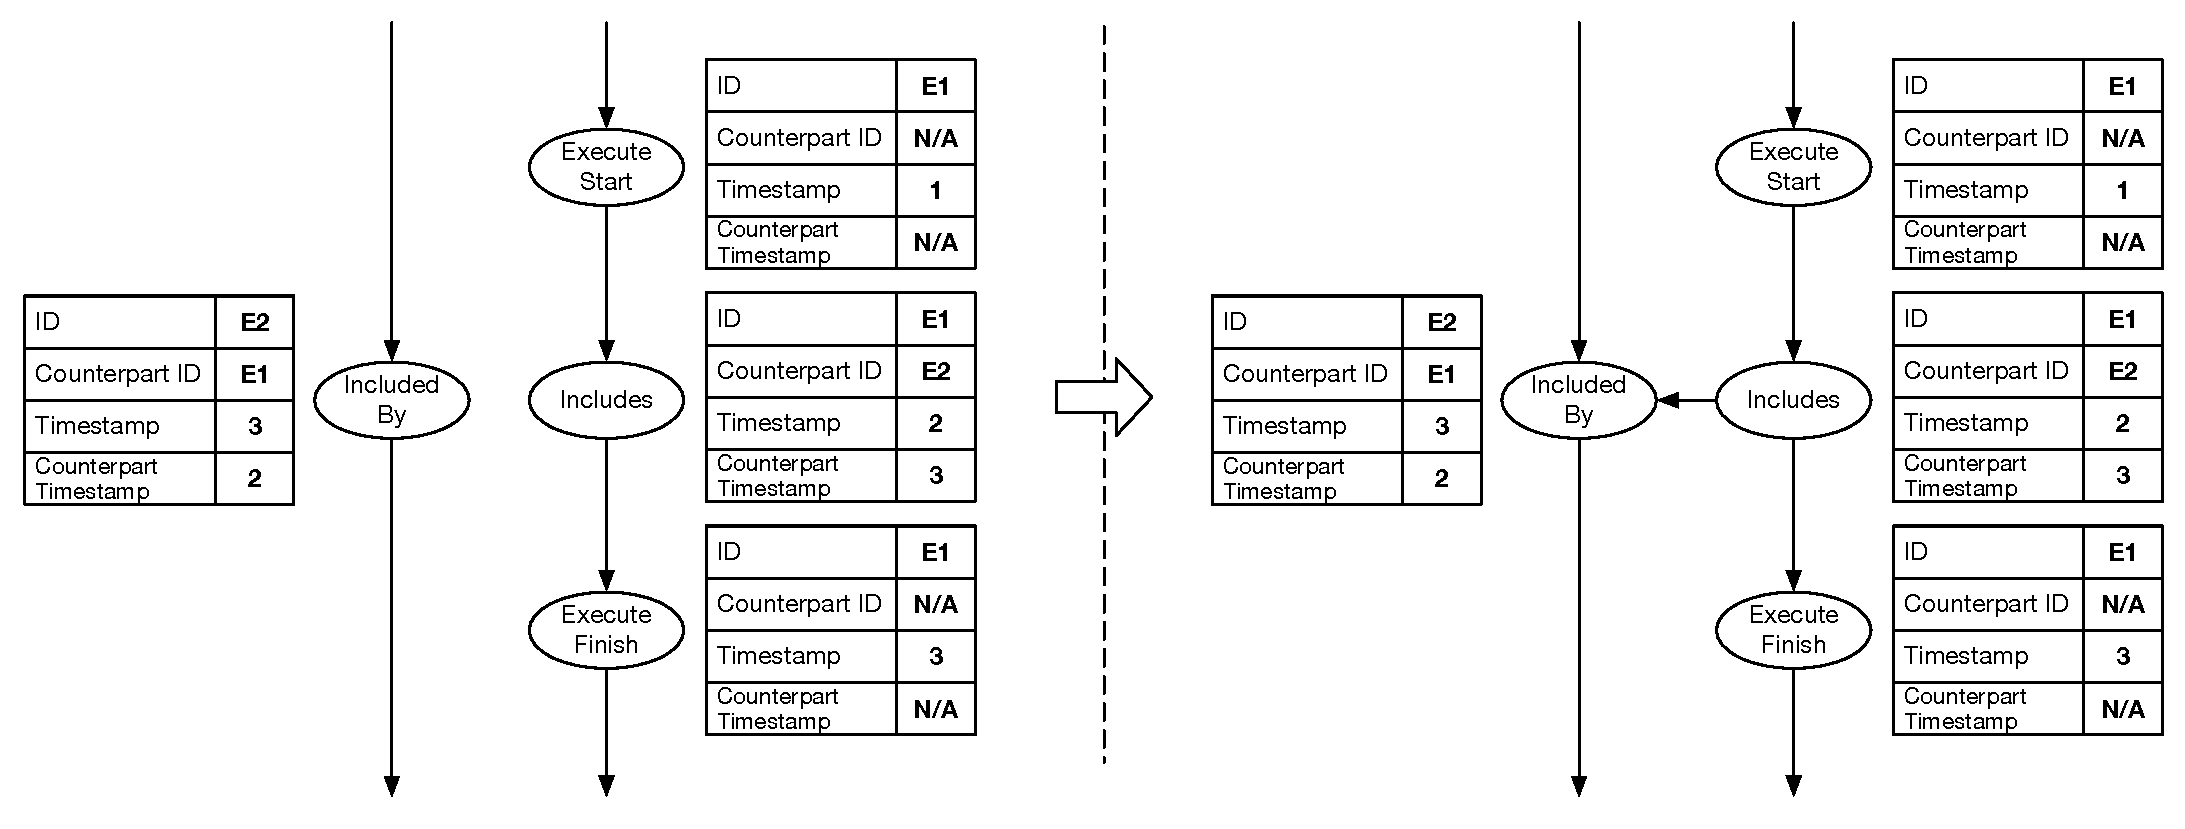
\includegraphics[width=\textwidth]{4connect/images/match-before-after.pdf}
		\caption{Actions of two merged histories before and after being matched.}
		\label{fig:connecting:match-before-after}
	\end{figure}
	
    \noindent In order to show that we have solved the problem of merging histories, we must show that all existing happens before relations of the local histories are still preserved and that we have added all of the possible happens before relations across histories.
    
    \newpar Since the method takes the union of all of the histories, which implies the union of all the action sets and happens before sets, and because no actions or happens before relations are removed, all the existing actions and happens before relations are preserved in the global history, which means that all paths in the local histories are present in the global history.
    
    \newpar Given that the union of all local histories contains the actions of every message exchange that has happened in the workflow and the algorithm have found all matching actions, corresponding to every message exchange, then every message exchange must be part of the global history. Because it is only possible to find happens-before relations across processes when they have exchanged a message, all happens-before relations between the histories of events must have been found.
    
    \newpar To explain why it is necessary to assume that all local histories are valid, we must first describe the implications of local histories being invalid. If we do not assume that all local histories are valid, it is not possible to assert that the union of the local histories contains all the actions and happens before relations between the actions that have happened, and therefore the global history will not be a representation of the actual global history of the workflow. This also means that we cannot assert that message exchanges, and actions in general, are not created, omitted, or changed. In the end, the algorithm could return an invalid global history if we do not assume that all local histories are valid.

    \section{Gathering of Local Histories}
    To merge the histories together it is necessary to acquire the local histories of the events of the DCR graph.
    \subsection{Gathering With a Central Server}
    In a central server system where the server has access to all the individual events, it is a trivial task to gather the histories. Simply request the server to get access to all the events and then request the histories of each event individually. This method is simple and only relies on the central server to get the addresses of all the events in the workflow. Furthermore the amount of messages sent to recieve all histories is $2N+2$ where N denotes the amount of events in the system. This is because the client has to send one message to the server and receive a response from it followed by a message exchange with each of the events. An illustration of this architecture is shown on \autoref{fig:connecting:server-contacts-events}.
    
    \begin{figure}[H]
    	\centering
    	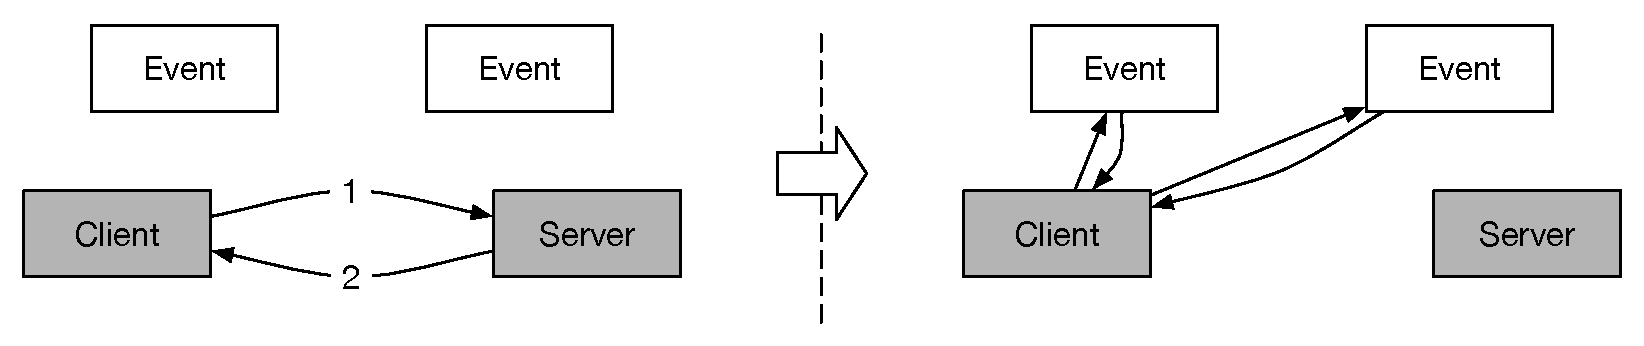
\includegraphics[width=\textwidth]{4connect/images/server-contacts-events.pdf}
    	\caption{The client requesting history from events and receiving it.}
    	\label{fig:connecting:server-contacts-events}
    \end{figure}
    
    \newpar Unfortunately, central server systems have drawbacks. E.g. if the server crashes or if it is busy processing other requests, then it is not possible to acquire the addresses of any of the events.
    
    Therefore it is desirable to create a peer to peer-based gathering algorithm, but this introduces a new set of challenges.
    
    \subsection{Gathering Without a Central Server}
    In order to use a peer-to-peer algorithm to gather history from a given workflow, it is necessary to study the structure of the distributed DCR graph.
    
    \newpar In distributed DCR graphs, events are connected only by their relations. Since there is no overall policy governing the placement of events on nodes in the network, a distributed DCR graph is unstructured. Therefore the only way of contacting events, is using recursive traversal of relations of events, and a single starting event must be known. The reachability of this event should preferably be the set of all other events in the workflow. If the reachability is a subset of all the events, then only a subset of all the local histories of the events can be gathered. Therefore the greater the reachability of the beginning event, the more complete the gathered history will be. This implies that it cannot not be guaranteed that the history of every event will be gathered if the DCR graph is not fully connected. This constitutes the first drawback of this approach.
	
	It is desired to develop an algorithm that, given an event with the desired reachability, is able to recursively gather all the local histories of the workflow. Since DCR graphs can contain cycles the algorithm also has to avoid endless recursion.
		
	\newpar Given a DCR graph where all events are reachable from the starting event, the algorithm should gather and merge the histories of each event in the graph into one global history.
	
	This is accomplished by recursively requesting the histories of neighbouring events and afterwards merging these histories with its own. To handle cycles, the use of a \textit{request trace} of previously contacted events is sent from each event to the next.
	
	\newpar When an event receives a request for its history, it subtracts all the events of the \texttt{request trace} from the set of the neighbours of the event. The result is the set of events to request history from. If this set is empty, the history of the event itself is returned. If the set is not empty the event sends requests to all of the events with its own ID appended to the \texttt{request trace}. When the event receives histories from its neighbours, it merges the histories and returns the merged history to the requester. The algorithm can be seen in \autoref{alg:produce} and a run of the algorithm is illustrated in \autoref{fig:connecting:recursive}.
	
	\begin{algorithm}[H]
		\begin{algorithmic}
			\State Event receives request for history with a \texttt{request trace}, $T$.
			\State
			\Function{Produce}{T, event}
				\State waitFor $\gets$ \Call{Minus}{event.Neighbours, $T$}\Comment{Subtract $T$ from neighbours.}
				\If {waitFor $= \emptyset$}
					\Return event.History
				\Else
					\State $T'\gets$\Call{Add}{event.Id, T}
					\State
					\State gatheredHistories $\leftarrow$ event.History
					\ForAll {$event'$ in waitFor} 
						\State history' $\leftarrow$ \Call{Produce}{$T'$, $event'$}\Comment{Requests history of $event'$ recursively}
						\State gatheredHistories $\leftarrow$ \Call{Merge}{history', gatheredHistories}
					\EndFor
					\State\Return gatheredHistories
				\EndIf
			\EndFunction
		\end{algorithmic}
		\caption{The \textit{\textbf{Produce}} algorithm}
		\label{alg:produce}
	\end{algorithm}
	
	\begin{figure}[H]
		\centering
		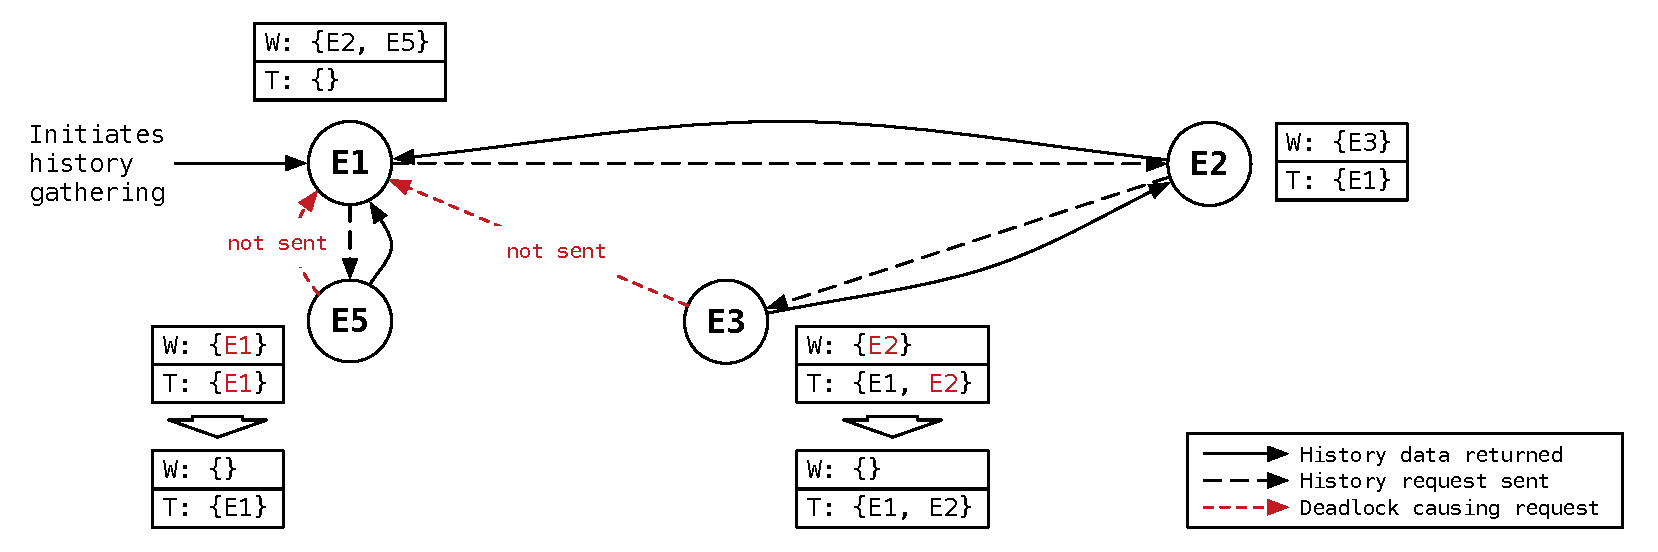
\includegraphics[width=\textwidth]{4connect/images/recursive.pdf}
		\caption{An illustration showing the recursive traversal the DCR graph seen on \autoref{fig:connecting:dcr-graph-cycle}. Note the avoidance of creating a deadlock.}
		\label{fig:connecting:recursive}
	\end{figure}
	
	\begin{figure}[H]
		\centering
		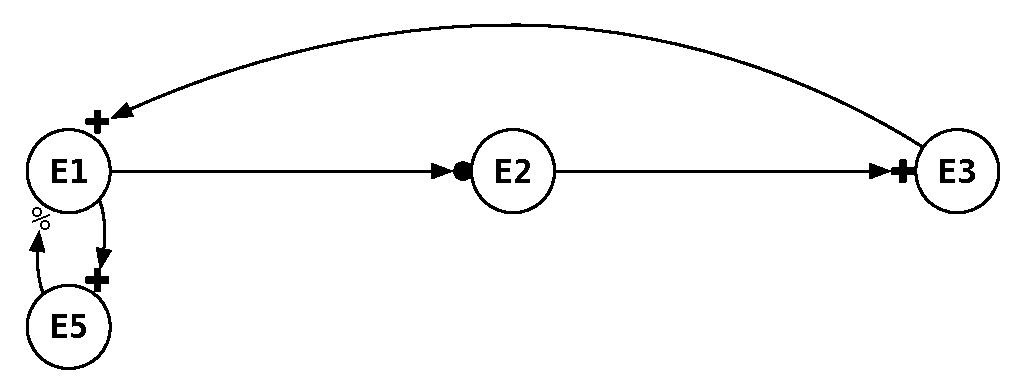
\includegraphics[height=0.15\textheight]{4connect/images/dcr-graph-cycle.pdf}
		\caption{An example of a DCR graph with cycles.}
		\label{fig:connecting:dcr-graph-cycle}
	\end{figure}
		
	\newpar This algorithm is in fact a modified version of the \textit{flooding search algorithm}, described in \cite{Coulouris:2011:DSC:2029110:chapter6}, for searching in unstructured peer-to-peer networks. Contrary to flooding, the produce algorithm not only returns the value at the searched for node, but returns every value at every reachable node. The flooding algorithm is often implemented with a time limit on the search and therefore does not care about cycles, which is handled more efficiently in the produce algorithm. Furthermore in the produce algorithm, every path to a node returns the value of that node.
	
	\newpar To argue that the produce algorithm correctly gathers all the local histories in the workflow we must show that every event is contacted. Since the algorithm contacts the neighbour of every contacted event, and the beginning event has a reachability of every event in the workflow, the set of contacted events must be all events in the workflow. If it is assumed that every event returns their history, as well as any recursively contacted event, then every history of the workflow must be returned to the beginning event. 
	
	The assumption that every event returns the history of every recursively contacted event, is unsafe in systems with Byzantine errors, which constitutes another drawback of the produce algorithm.
	
	\subsubsection*{Issues with the Produce Algorithm}
	If malicious processes are introduced in the DCR graph, the problem similar to not having full reachability from the beginning event arise. If the path to a given event, goes through an event on a malicious process, then that malicious process can either add, remove or change the history. That implies that any history retrieved from that event, might not be valid. The effects of this malicious behavior is worsened if the path to a great number of events goes through a malicious process. An illustration of this effect is shown in \autoref{fig:connecting:recursive-evil-node}. If there exists no path to an event that does not go through a malicious process, then the beginning node will potentially not have any valid version of that history. Even if it is possible to assert that the history is invalid, it is not possible to identify which event along the path has acted maliciously.
	
	\newpar Furthermore, this uncertainty is amplified because for each contacted event with lacking information, it is possible to tamper with the history of the recursively called events, or even add history of non existing events. Therefore some action must be taken to handle these pitfalls.
	
	\newpar One way to handle processes changing and adding histories of other events is to sign the histories before returning them to the requester. This is the approach to solve the Byzantine Generals Problem. Since the process starting the produce algorithm, does not know the address of all events, then it is possible for other processes to sign changed or added histories with its own certificate, and tell anyone who want to confirm the certificate to contact the malicious process itself. In order for these certificates to be effective, all processes must therefore know the certificate or location of any other process in the system.
	
	\newpar If the certificates of all processes are known beforehand, a security breach would leave the entire system open for attacks. On the other hand, if the addresses of all events are known, then we have a situation where the central server algorithm is sufficient, because certificates of messages are no longer required, under the assumption that man-in-the-middle attacks does not occur.
	
	\begin{figure}[H]
		\centering
		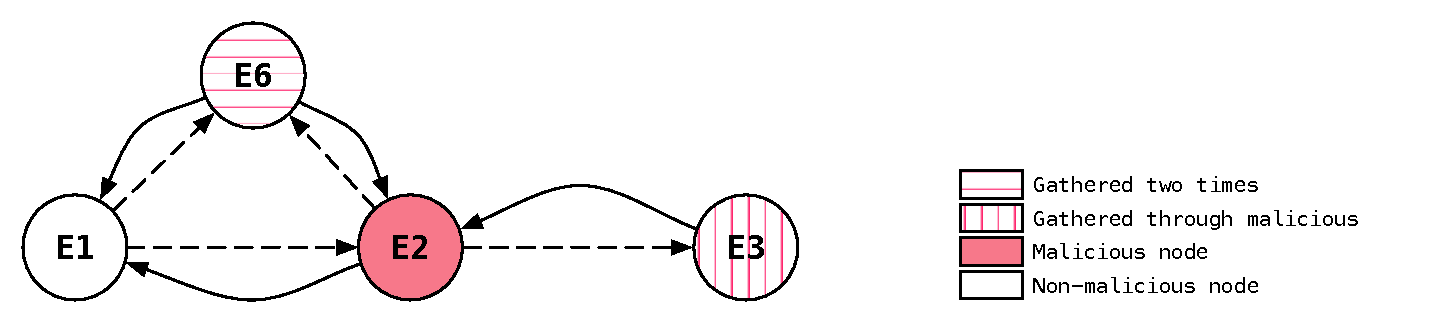
\includegraphics[width=\textwidth]{4connect/images/recursive-evil-node.pdf}
		\caption{A malicious node in a graph. Note that it is not possible to ensure that any history passing through the malicious node is valid.}
		\label{fig:connecting:recursive-evil-node}
	\end{figure}
	
	\noindent The produce algorithm sends an exponential number of messages in the amount of events in the worst case. Redundant history from every path from a given node to any other reachable node is wanted. This is the reason that the complexity is exponential. The worst case is when the graph is fully connected and every node therefore has an edge to any other node. High connectivity in the graph is a wanted property since it allows for better validation of the histories. This is explained in \autoref{chap:validation}.
	
	\newpar Caching history produced of an event before transferring it to a requesting event could improve performance, but presents a new problem. This problem is most easily illustrated with a figure. In \autoref{fig:connecting:caching} we have a situation where 4 events, $A$, $B$, $C$, and $D$ gather histories. The numbers on the arrows in the figure represent the order in which messages are sent. $A$ starts by contacting $B$, which in turn contacts $C$ which contacts $D$. $D$ returns its local history to $C$ because $B$ is already part of the trace. $C$ then caches the result of $D$ and its local history. $C$ then returns the history to $B$ which caches the result along with its local history. $B$ returns the history to $A$, which can then contact $C$ for its history. When $C$ is contacted, it just returns its cached history, which does not contain the history of $B$. The history of $B$ can therefore not be confirmed on multiple paths.
	
	\begin{figure}[H]
		\centering
		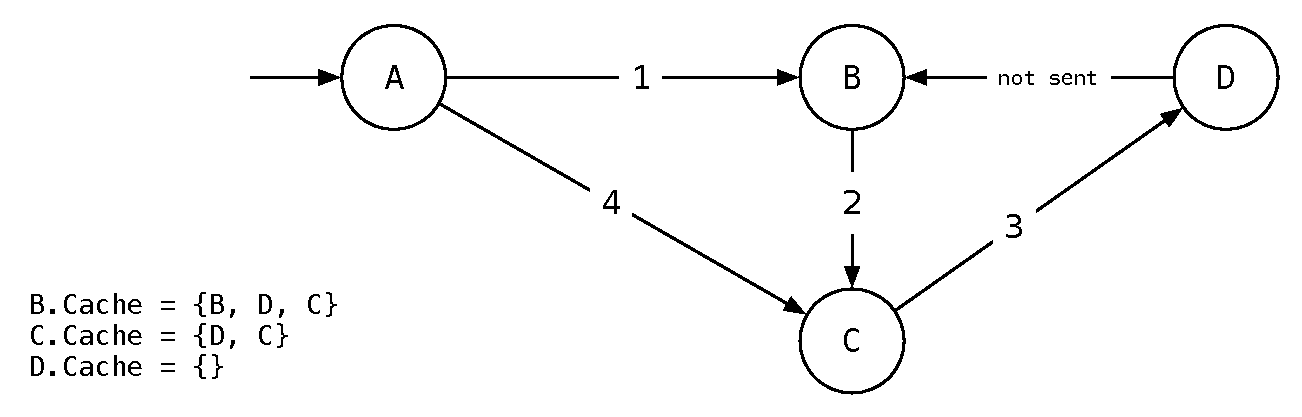
\includegraphics[height=0.20\textheight]{4connect/images/caching.pdf}
		\caption{An example of a recursive gathering where caching would result in a incomplete history being returned.}
		\label{fig:connecting:caching}
	\end{figure}
	
	\noindent There might be solutions to the presented issues, but these have not been examined further in this project. Because of the problems presented in this section, we have chosen to use the central server gathering algorithm.